%; whizzy chapter
% -initex iniptex -latex platex -format platex -bibtex jbibtex -fmt fmt
% 以上 whizzytex を使用する場合の設定。

%     Kansai Debian Meeting resources
%     Copyright (C) 2007 Takaya Yamashita
%     Thank you for Tokyo Debian Meeting resources

%     This program is free software; you can redistribute it and/or modify
%     it under the terms of the GNU General Public License as published by
%     the Free Software Foundation; either version 2 of the License, or
%     (at your option) any later version.

%     This program is distributed in the hope that it will be useful,
%     but WITHOUT ANY WARRANTY; without even the implied warranty of
%     MERCHANTABILITY or FITNESS FOR A PARTICULAR PURPOSE.  See the
%     GNU General Public License for more details.

%     You should have received a copy of the GNU General Public License
%     along with this program; if not, write to the Free Software
%     Foundation, Inc., 51 Franklin St, Fifth Floor, Boston, MA  02110-1301 USA

%  preview (shell-command (concat "evince " (replace-regexp-in-string "tex$" "pdf"(buffer-file-name)) "&"))
% 画像ファイルを処理するためにはebbを利用してboundingboxを作成。
%(shell-command "cd image200708; ebb *.png")

%%ここからヘッダ開始。

\documentclass[mingoth,a4paper]{jsarticle}
\usepackage{kansaimonthlyreport}
\usepackage[dvips]{xy}

% 日付を定義する、毎月変わります。
\newcommand{\debmtgyear}{2012}
\newcommand{\debmtgdate}{28}
\newcommand{\debmtgmonth}{10}
\newcommand{\debmtgnumber}{65}

\begin{document}

\begin{titlepage}

% 毎月変更する部分、本文の末尾も修正することをわすれずに

 第\debmtgnumber{}回 関西 Debian 勉強会資料

\vspace{2cm}

\begin{center}
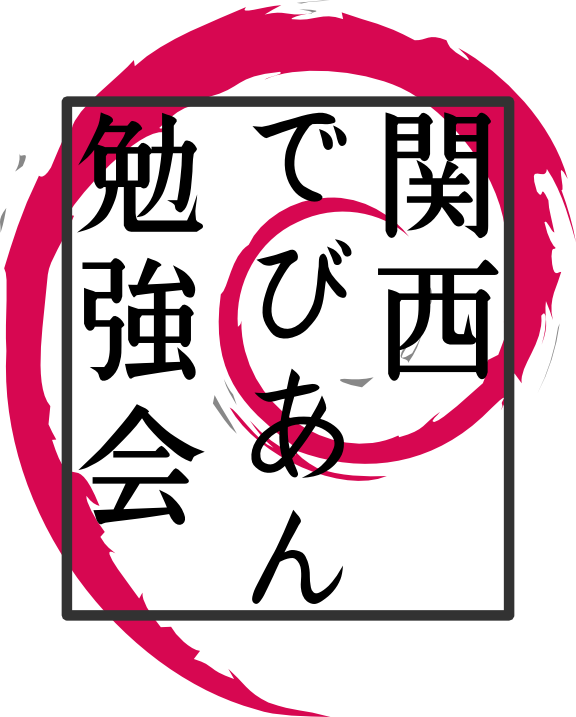
\includegraphics{image200802/kansaidebianlogo.png}
\end{center}

\begin{flushright}
\hfill{}関西 Debian 勉強会担当者 佐々木・倉敷・のがた・かわだ \\
\hfill{}\debmtgyear{}年\debmtgmonth{}月\debmtgdate{}日
\end{flushright}

\thispagestyle{empty}
\end{titlepage}

\dancersection{Introduction}{Debian JP}

 関西Debian勉強会はDebian GNU/Linuxのさまざまなトピック
 (新しいパッケージ、Debian特有の機能の仕組、Debian界隈で起こった出来事、
 などなど)について話し合う会です。

 目的として次の三つを考えています。
 \begin{itemize}
  \item MLや掲示板ではなく、直接顔を合わせる事での情報交換の促進
  \item 定期的に集まれる場所
  \item 資料の作成
 \end{itemize}

 それでは、楽しい一時をお楽しみ下さい。

\newpage

\begin{minipage}[b]{0.2\hsize}
 {\rotatebox{90}{\fontsize{80}{80}
{\gt 関西 Debian 勉強会}}}
\end{minipage}
\begin{minipage}[b]{0.8\hsize}
\hrule
\vspace{2mm}
\hrule
\setcounter{tocdepth}{1}
\tableofcontents
\vspace{2mm}
\hrule
\end{minipage}

\dancersection{最近のDebian関係のイベント報告}{Debian JP}

\subsection{第 64 回関西 Debian 勉強会}

64 回目の関西 Debian 勉強会は 9 月 23 日に福島区民センターで行ないました。

「clangによるパッケージビルド」と「月刊 Debian Policy 文書」でした。

普段 Debian 使いでない方の Debian Policy 解説、他のディストリビューションとの違いなどいつもと違った切り口もあってよい内容ではなかったでしょうか。


\subsection{第 93 回東京エリア Debian 勉強会}
93 回目の東京エリア Debian 勉強会は 10 月 20 日に開催されました。

「Haskell の Debian packaging 周辺について語ります」、「レゴでなめこ収穫期」、「xf86-input-mtrack」といった内容でした。

レゴでどうやってなめこ収穫を?と興味を持たれた方は今月の東京エリア Debian 勉強会の資料を参照してください。



\dancersection{事前課題}{Debian JP}

今回は以下の課題を出題しました.
\begin{screen}
  \begin{enumerate}
  \item poEdit など、使用した事がある翻訳支援ツールの概要・長所・短所を教えて下さい。

    po4a や 自作のスクリプトなどでも結構です。

    翻訳に参加したことが無い方やツールを使用しない方は、何か1つ翻訳支援ツールについて調べ、概要・長所・短所を教えて下さい。

  \item 今年八月以降のDSAを一つ選び、英語の原文と日本語訳を読み比べて、翻訳に関して忌憚なく批評して下さい。

    DSA は、ML debian-security-announce@lists.debian.org と debian-users@debian.or.jp のバックナンバーを読むか、
    \url{http://www.debian.org/security/} あるいは \url{http://www.debian.org/security/2012/} の web ページで探すことができます。

  \end{enumerate}
\end{screen}

参加者の皆さんの解答は以下の通りです。


\begin{prework}{ munepixyz }
未回答

\end{prework}

\begin{prework}{ かわだてつたろう }
\begin{enumerate}
\item 翻訳はしたことがありません。翻訳支援ツールについて調べられていません。
\item 日本語としてこなれていなかなと思うことがあります。
\end{enumerate}
\end{prework}


\begin{prework}{ 川江 }

\begin{enumerate}
\item OmegaT Javaで記述されたコンピューター翻訳支援ツール
\item DSA-2567-1 request-tracker3.8 -- 複数の脆弱性を見比べました。特になし。
\end{enumerate}

\end{prework}

\begin{prework}{ 木下 }

\begin{enumerate}
\item 私がよく使うのは、インフォシークのWeb翻訳サイトです。
\begin{description}
\item [長所]:
\begin{itemize}
\item 電気代除いてコスト0円
\item 大まかな意味の理解がお手軽にできる。
\end{itemize}
\item [短所]:
\begin{itemize}
\item まったく意味不明な翻訳となることがある。
\item 翻訳の結果を信用できない
\end{itemize}
\end{description}

\item 正直、英語はできない人なので、よくわかりません。
\end{enumerate}

\end{prework}

\begin{prework}{ yyatsuo }

\begin{enumerate}
\item OmegaT と vim をいったりきたりしています。OmgaT で訳す前の下処理と後処理を自作のPythonクスリプトで行っています。

\item 特にどれというわけではありませんが、指示語が何を指しているのか(もちろん文意から明らかな場合が多いですが)いまいちはっきりしない場合が多い気がします。
\end{enumerate}

\end{prework}

\begin{prework}{ 岡野孝悌 }

\begin{enumerate}
\item Ubuntu 12.10 Quantal Quetzal のリリースノートを翻訳した際(http://togetter.com/li/392260 さんしょ)、松澤さんが txt2po を使って wiki テキストを po に変換して作業していたので、まねしてみた。
translate-toolkit の一部で、テキストと po の変換ができる (po4a みたいに使える)。
Ubuntu Wiki の wiki テキストは改行が CRLF で、txt2po では問題ないのだが、po2txt でテキストに戻すときにハマった。(複数行からなるメッセージをうまく処理してくれない)

\item
  \begin{itemize}
    \item dsa-2531.wml の以下の訳がよくわからない。
    \item
      \begin{description}
        \item [原文:] Since this can be used to crash a client from within, this vulnerability is considered to have low impact.
        \item [訳:] このことは使われてもそのクライアントを内部から異常終了させるためになるので、この脆弱性は低い影響力しかないとみなされています。
      \end{description}
    \item 句読点は「、。」を使う方針のようだが、理系読点 (dsa-2533.wml,dsa-2534.wml,dsa-2537.wml,dsa-2541.wml,dsa-2548.wml,dsa-2557.wml) や、理系句点 (dsa-2536.wml) がある。
    \item dsa-2540.wml 「符号化ていない」は「符号化していない」の誤り。
    \item dsa-2555.wml malformed document を「形の崩れた文書」と訳しているのが引っかかる。
  \end{itemize}
\end{enumerate}

\end{prework}

\begin{prework}{ 西山和広 }

\begin{enumerate}
\item gettext-el
\begin{description}
\item [概要:] emacs の po ファイル編集用モード
\item [長所:] emacs の編集機能が使える
\item [短所:] msgstr ごとに編集するので po ファイル全体に一括置換したいなどの操作には向かない
\end{description}

\item http://www.debian.org/security/2012/dsa-2557 に「バッファオーバフロー」と「バッファオーバーフロー」の表記揺れがあります。
http://www.debian.org/security/2012/dsa-2556
「繋がりかねません。」よりも昔の DSA の翻訳にあるように「繋がる恐れがあります。」の方がわかりやすいように思います。
\end{enumerate}

\end{prework}

\begin{prework}{ 末廣 雅利 }

\begin{enumerate}
\item Google Translator Toolkit (+ Chrome + 英辞郎 on the WEB プラグイン)
とある業界団体で RFC の翻訳を共同で行なった際に Google Translator Toolkit を利用した。

\begin{description}
\item [概要:] Google Translator Toolkit は Google が無料で提供している翻訳のための Web サービスである。ファイルをアップロードしたり、URL を指定することによって原文を取り込むことができる。Google 翻訳による下訳が自動的に行われ、上手くはまるとビックリするくらいよい訳がつくことがある。同一の文章で以前に人間によって翻訳された例があると、下訳や訳の候補に反映される。
\item [長所:]
\begin{itemize}
\item 自動的に下訳が行われるため、参考になることがある。
\item Web サービスであるため、共同作業がしやすい。
\end{itemize}
\item [短所:] 原文の文章の書式によっては自動翻訳の際に文の区切りが正しくなくて、下訳が意味をなさないことがある。
\end{description}

\item DSA の翻訳について
\begin{itemize}
\item 昔(10年ぐらい前) と比較するとかなりこなれた訳になっていると思います。
\item セキュリティ業界でみかけるのとはちょっとズレている言い回しがあるような気がして少し違和感を覚えることがあります。
\end{itemize}
\end{enumerate}

\end{prework}

\begin{prework}{ 佐々木洋平 }
\begin{enumerate}
\item Emacs の gettext-mode ぐらいです。いまだに使い方よくわからないな。

\item お疲れ様です。
\end{enumerate}
\end{prework}

\begin{prework}{ のがたじゅん }

\begin{enumerate}
\item 最近Qtアプリを翻訳するときにlinguistを使いました。
フレーズブックで用語集が使えるのは便利ですね。同じ機能は他にもあると思いますがQt付属のフレーズブックがあって、それを使うとQtアプリなら最低限言葉が揃うのはいいなと思いました。(メニューなど本当に基本的なところだけですが…)
あと、GUIアプリにありがちなフレーズがメニューのどこにあるかが、実際のフォームを見ながら確認できるのは便利だと思いました。
短所は、linguistは基本的にQtの翻訳のためのアプリなので、gettext対応がオマケな事でしょうか。

\item DSA-2560-1 bind9 -- サービス拒否
http://www.debian.org/security/2012/dsa-2560.en.html
http://www.debian.org/security/2012/dsa-2560.ja.html
「DNS サーバである BIND に、 リソースレコードの特定の組み合わせが存在する場合 DNS 応答の追加セクション構成時にハングすることが発見されました。」

意味は分かるのですが、日本語的にこなれていないような気がします。
\end{enumerate}

\end{prework}

\begin{prework}{ jmatsuzawa }

\begin{enumerate}
\item 短所:ヘッダーやフォーマットを勝手にいじられる、そのためバージョン管理に不都合がでる。

\item
「this problem has been fixed in version 〜」というのを、「この問題はバージョン 〜 で*修正されています*」と訳すのではなく、「...で修正済みです」あるいは「...で修正されました」とした方が良いと思います。
「修正されています」だと、「鋭意修正中」なのか「既に修正された」のかどちらでも解釈できてしまうので。雰囲気でなんとなくわかりますが、重要な情報では両義性を残さないのが無難だと思います。
\end{enumerate}

\end{prework}

\begin{prework}{ 山城の国の住人 久保博 }
\begin{enumerate}
\item OmegaT を使用したことがあります。
\begin{description}
\item [長所:] 近い参考訳文と略語が自動的に表示されること。自動保存機能。
\item [短所:] 文書を編集する機能が弱いこと。翻訳対象の取り込み間違いを取り消すのが無理(やり方を知らないだけ?)なこと。原文ファイルを管理する機能が貧弱なので、一つのプロジェクトにたくさんの原文ファイルを登録すると、原文ファイルを探すのが大変。参考訳文の機能があと一歩機能的に足らないので、実際には使っていません。惜しい感じがします。
\end{description}

\item heap-based buffer overflow に対する訳語がブレすぎです。ちなみに適訳が未だに分かりません。
\end{enumerate}

\end{prework}

\begin{prework}{ lurdan }

例によって遅刻して後半に参加予定です。

\begin{enumerate}
\item Emacs
翻訳専用の環境におまけでついてる貧弱な編集機能に足をひっぱられることなく、まともな編集環境で自分が必要な翻訳サポートを取捨選択することができます。一文単位の翻訳なら rosetta でいいやと思うけど、長文を訳すなら Emacs でないと辛いですね。

\item bacula (http://www.debian.org/security/2012/dsa-2558)
> コンソールの ACL を適切に実施していないことが判明しました。

「ACL を実施」という表現はあまり使わないような気がするので、
「コンソールの ACL を正しく強制しないことが判明しました」とか。

> 本来制限を受けるはずのクライアントによって計算機資源に関する情報がダンプされることを許しかねません。

ACL (アクセス制御) が正しくない、ということなので、resouce は「bacula サーバが保持しているバックアップについてのデータ」という位置付けになるかと思います。なので単に「リソース」でよさそうです。あとは、ちょいと固いので

「このため、本来なら制限されていたはずのクライアントがリソース情報をダンプできてしまう可能性があります」

とか?
\end{enumerate}

\end{prework}


\clearpage

\dancersection{本気で "使える" 翻訳環境を構築してみた(い)}{八津尾}
\subsection{はじめに - 今日の主旨}
アプリケーションのローカライズに man ページ、wiki 等々、普段何気にお世話に
なっている翻訳ですが、OSS の世界では (当然ですが) 有志によって行われています。
しかし、日本の OSS コミュニティにおいて翻訳者の不足はどのプロジェクトでも共通
の課題らしいということをよく耳にします。翻訳は高い技術力を必要とせず、誰でも簡
単に参加できます。翻訳支援ツールを使い、翻訳のプロセスを簡略かつ明確にすること
で、さらに参加する為の敷居が下がるのではないでしょうか?ということで、翻訳ツー
ルを利用した翻訳環境の構築事例を紹介していきたいと思います。

今回は翻訳ネタ2本立てという事で、トランスレータとして各プロジェクトに参加中
の皆さん、またこれから翻訳に参加してみようかとお考えの皆さんと一緒に、
翻訳環境について議論していきたいと思いますので積極的な発言をお願いします。

\subsection{DPN の翻訳効率化}
Debian Project News (以下、DPN ) の翻訳に参加しはじめてから半年が過ぎま
した。DPN を翻訳していくなかで、いくつか気づいた事があります。

\begin{itemize}
    \item ほぼ同じ内容の文章を何度も訳している
    \item 担当者が過去記事を参照せず、同一の事象での訳語が統一できていない
    \item グロッサリが存在せず、担当者間で訳語が統一できていない
    \item 明確なスタイルガイドラインが存在せず、暗黙のルールで運営されている
    \item 過去に訳した膨大な量の訳文 (=資産) を活かしきれていない
\end{itemize}

このような無駄を無くし、翻訳を効率化するために{\tt 翻訳メモリ}が活用できるの
ではないかと考え、現在快適な翻訳環境作りに取り組んでいるころです。私が考える
翻訳環境の柱は次のようになります。

\begin{itemize}
    \item 訳語を意識せずに揃えること
    \item 誰が翻訳しても同一の品質を保てること
    \item 過去の翻訳結果を再利用できること
    \item 翻訳プロジェクトのメンバ内でこれらの結果を共有できること
\end{itemize}

\subsubsection{翻訳メモリとは?}
{\tt 翻訳メモリ}とは、"ソースの言語とターゲットの言語を 1 対 1 で保存した
データベースのようなもの"です。
{\tt 翻訳メモリツール}は、翻訳メモリから類似の文章を探し出しヒット率が高い
文章の訳文を提示したり自動挿入や置換をする事で翻訳の支援を行うツールです。

よく勘違いされるのですが、{\tt 翻訳メモリツール}は勝手に翻訳してくれる機械翻
訳のようなものではありません。{\tt 翻訳メモリ}は自分で育てる必要があり初期状
態では全く使いものになりません。また、{\tt 翻訳メモリツール}は訳文の正確性の
判断はできないので、翻訳メモリに誤訳が混入しそれが繰り返し利用されてしまう可能
性がある事を常に念頭に置いておきましょう。

{\tt 翻訳メモリ}には{\tt TMX (Translation Memory eXchange)}という
XML ベースの規格があり、広く利用されています。
\footnote{もともと LISA (Localization Industry Standards Associa
	tion) によって策定された規格。2011年、LISA は破産宣告によって解散し、
	LISA で策定された他の規格と共にパブリックドメインへと帰した。}

産業翻訳でデファクトスタンダードとなっている
{\tt SDL TRADOS \textregistered}\footnote{http://www.trados.com}
や、本セッションで紹介予定の {\tt OmegaT}
\footnote{http://www.omegat.org} もこの{\tt TMX}を採用しています。
{\tt 翻訳メモリ}の更に詳しい概要と {\tt OmegaT} の操作方法については、
2011 年 10 月の関西 Debian 勉強会資料に掲載されている拙著「翻訳で Debian
に貢献しよう」も参考にしてください。

\subsubsection{定型記事と翻訳メモリ}
翻訳メモリがその真価を発揮できるのが、ある程度定型化された記事を
翻訳する場合です。以下の文例を見て下さい。

\begin{itembox}[c]{DPN2012 issue 15 より}
    \begin{verbatim}
<toc-add-entry name="newcontributors">New Debian Contributors</toc-add-entry>
	<p>
    Seven applicants have been
    <a href="https://nm.debian.org/public/nmlist#done">accepted</a>
    as Debian Developers, nine applicants have been
    <a href="http://lists.debian.org/E1Sta5X-0005lb-Ap@franck.debian.org">accepted</a>
    as Debian Maintainers, and six people have
    <a href="http://udd.debian.org/cgi-bin/new-maintainers.cgi">started to
    maintain packages</a> since the previous issue of the Debian Project News.
    Please welcome (著者注:中略 ここで人名が列挙される) into our project!</p>
    \end{verbatim}
\end{itembox}
\begin{itembox}[c]{DPN2012 issue 17 より}
    \begin{verbatim}
<toc-add-entry name="newcontributors">New Debian Contributors</toc-add-entry>
	<p>
    Three applicants have been
    <a href="https://nm.debian.org/nmlist.php#newmaint">accepted</a>
	as Debian Developers,and two people have
    <a href="http://udd.debian.org/cgi-bin/new-maintainers.cgi">started to
    maintain packages</a> since the previous issue of the Debian Project News.
    Please welcome (著者注:中略 ここで人名が列挙される) into our project!</p>
    \end{verbatim}
\end{itembox}

これらの記事はほぼ同じ内容であり、毎月必ず掲載される記事です。にも関わらず、
Debian-www メーリングリストで配布される原文に添付されている、おそらく何かの
スクリプト処理によって生成されたと思われる試訳では全く訳されません。翻訳メモリ
で一度でも訳しておけば、以降は訳文候補として過去の訳が参照できるのでこのような
記事をシームレスに翻訳することができます。では、実際に {\tt OmegaT} でどの
程度効率化できるのか試してみましょう。なお、ここでは {\tt OmegaT} の詳しい
使い方は説明しませんが、起動時に表示されるお手軽スタートガイドに目を通すだけで
一通りの作業はこなせるようになるでしょう。

\begin{itembox}[l]{DPN2012 issue 15 の日本語訳}
    \includegraphics{image201210/omegat_demo1.eps}
\end{itembox}

\begin{itembox}[l]{DPN2012 issue 17 を訳しているところ}
    \includegraphics{image201210/omegat_demo2.eps}
\end{itembox}

このように、翻訳メモリを利用することで訳語の揺れを減らし訳文の品質を高めること
ができます。

\subsubsection{訳語の統一}

担当者が変わったり単に翻訳者が以前当てた訳語を忘れてしまい、訳語から統一感が失
われてしまうという問題はしばしば発生します。この問題に対処する為にはグロッサリ
のメンテが必要不可欠です。

訳語を決めたらグロッサリに登録しておきましょう。{\tt OmegaT} の場合は UTF-8 の
タブ区切り形式でグロッサリを作成しておくことができます。
\footnote{複合語に難があったりとあまり洗練されていない}
残念ながら、現在メンテされていませんが{\tt OmegaT} で利用できる Debian 翻訳用
のグロッサリも入手可能です。
\footnote{Debian JP Doc/WWW 対訳表:http://www.debian.or.jp/community/translate/}
私は現在個人でグロッサリの作成とメンテをしていますが、本来であればプロジェクト
単位で準備すべきものです。グロッサリを整備しておくことで、新規参入者が迷わずに
翻訳を始められるのではないでしょうか。

\subsubsection{マークアップと翻訳メモリ}
DPN は {\tt wml} という {\tt html} によく似た {\tt xml} の拡張フォーマットで
記述されたものがメーリングリストで配布され、それを各担当者が訳しています。
{\tt OmegaT} を利用する時に注意が必要な事は、{\tt wml} がサポートされていない
という事です。
{\tt OmegaT} でサポートされていないファイルフォーマットは翻訳対象ファイルから
見えません。他にも、古いドキュメント類に散見される {\tt sgml} などはサポート
されていないので、ちょっとしたトリックでこれを翻訳できるようにしましょう。

もっとも簡単な方法はテキスト形式にしてしまうことです。翻訳対象ファイルの拡張子
を *.txt にしても良いですし、*.txt のファイルフィルタに翻訳したいファイルを登
録する方法もあります。しかしこの方法を使うと、タグの中まで翻訳対象となってしま
い翻訳メモリの能力を最大限引きだす事ができません。テキスト形式にしてしまう前に、
近いフォーマットのフィルタを試してみると良いでしょう。
私は {\tt wml} に {\tt html} のフィルタを使用しています。いまのところ
問題なく使えています。
\footnote{OmegaT の Okapi プラグインで対応ファイルを増やす方法もある}

\subsubsection{翻訳ツール}
翻訳メモリを導入することで、私が必要としていることの大半は実現できましたが、
理想の環境とはほど遠いのが現状です。まだまだ試行錯誤の段階では
ありますが、私が現在 DPN の翻訳に使用しているツールを紹介します。

\begin{itemize}
\item DPNToolKit.py -
	自作の python スクリプトです。{\tt wml} ファイルを分解し {\tt OmegaT}
	 のプロジェクトフォルダに配置したり、{\tt OmegaT} が生成した訳文から
	査読メール用の文章を生成したりします。
\item Debian JP Doc/WWW 対訳表
    一応導入し、個人的にメンテしています。{\tt OmegaT} から参照可能です。
\item 英辞郎 -
    言わずと知れたオンライン辞書です。第3版とオンライン版を適宜使い分けていま
    す。{\tt OmegaT} から参照可能です。
\item Google翻訳 -
    私が知っている機械翻訳の中で、最も精度の高い翻訳結果を出すのが Google翻訳
    です。機械翻訳はあくまで参考に使用する程度にしましょう。
\item vim -
    ちょっとした文章は vim で訳してしまうことが多いかも。
    W3m プラグインで英辞郎や WikiPedia を参照でき、重宝しています。
    OmegaT の外部エディタとして vim や emacs が使えれば最高なのですが…
\item translate-toolkit -
    今後使用してみたいツール群です。特に {\tt po2tmx} が気になっています。
    {\tt po} ファイルから {\tt tmx} 形式の翻訳メモリを生成できます。これ
    を活用すれば、ソフトウェアのローカライゼーションが一気に楽になるのではな
    いでしょうか?
\end{itemize}

\subsection{今後の課題}
\begin{itemize}
    \item 翻訳メモリをプロジェクト内で共有する方法
    \item OmegaT の残念なインタフェースをどうするか
    \item OmegaT 以外翻訳メモリを調査する
    \item GlobalSight について調査する
    \item 翻訳スタイルガイドラインみたいなもの作りたい
\end{itemize}
\clearpage

\dancersection{Debian セキュリティ勧告翻訳の舞台裏}{山城国の住人 \  久保博}
\newcommand{\email}[1]{{\tt{}#1}}
\subsection{はじめに}

Debian セキュリティ勧告の翻訳に携わるようになったので、Debian セキュリティ勧告の簡単な紹介を交えながら、その翻訳の過程がどのようになっているか、紹介します。

\subsubsection{Debian セキュリティ勧告}

Debian セキュリティ勧告 (Debian Security Advisory 以下略称 DSA を使う)は、
Debian を構成するソフトウェアのセキュリティに関する問題を公開し、対策を勧める文書です。
Debian セキュリティチームの構成員が執筆しており、DSA- で始まる通し番号が振られ、執筆者のデジタル署名付のメールで \email{debian-security-announce@lists.debian.org} メーリングリストに発表されています。

また、「Debian 安全化マニュアル」の2.3節\cite{securehowto2.3}によれば、そもそも DSA を発行することは、Debian 社会契約\cite{socialcontract}の第三項「私たちは問題を隠しません」の具体的な取り組みの一つです。

日本では、その日本語訳を \email{debian-users@debian.or.jp} メーリングリスト (以下、略して \email{d-u}) に流す取り組みが以前から継続してなされています。


\subsubsection{日本語訳作業への参加の経緯}

今年(2012年)7月まで翻訳を \email{d-u} に流されていたかねこさんが、しばらくの間インターネット接続が途切れるので翻訳を流すことが滞る旨の予告を \email{debian-www} メーリングリストで流されました。
それを受けて、中断期間中に筆者が翻訳を始めました。その後、かねこさんがインターネット接続が復帰とともに、翻訳活動を引退される旨のメールが流れたので、引続き筆者がDSA の翻訳活動を努めるようになりました。
現在、筆者一人で活動しています。


\subsection{翻訳作業}

\subsubsection{環境作り}

Debian パッケージ中心で翻訳作業環境を整えています。

\paragraph{翻訳文編集環境用のパッケージ}

\begin{description}
\item[emacs23] GNU Emacs
\item[sed] 定型文の置換処理のスクリプト用.
\item[omegat] Computer Assisted Translation (CAT) tool. OmegaT
\end{description}

また、辞書もパッケージにあるものはインストールしてあります。

\paragraph{辞書パッケージ}
\begin{description}
\item[dict-gcide] A Comprehensive English Dictionary
\item[dict-jargon] dict package for The Jargon Lexicon
\item[dict-moby-thesaurus] 最大かつ最も理解しやすい類語辞典
\item[edict] English / Japanese dictionary
\end{description}

更にこれらの辞書を引くために、次のパッケージをインストールして使っています。
\paragraph{辞書利用環境のパッケージ}
\begin{description}
\item[lookup-el] emacsen での電子辞書インターフェイス
\item[ndtpd] ネットワークディレクトリ転送プロトコルサーバ
\item[ebnetd] the server of EBNET protocol
\end{description}


\subsubsection{事前準備}

電子メールで DSA を受信するために、\email{debian-security-announce} メーリングリストを購読します\footnote{メーリングリストの購読方法は \url{http://lists.debian.org/debian-security-announce/} を参照。}。

また、DSA のメールは、セキュリティチームの構成員のPGP署名が付与されています。これを検証することで、セキュリティチームからの正式な発表であることが確認できますので、電子メールの PGP 署名を検証できるようにしておきます。gnupg パッケージをインストールしておくと良いでしょう。



\subsubsection{DSA受信から翻訳文送信まで}

DSAを受信してから、 \email{d-u} に流すまでが、DSA翻訳として受け持っている作業です。
大まかに分けると、次のような段階を踏んで作業しています。

\begin{enumerate}
\item DSA の受信と署名の検証
\item DSA 本文の翻訳
\item \email{debian-users@debian.or.jp} メーリングリストへの投稿
\item 後処理 難訳語の用語集への登録など
\end{enumerate}

\subsubsection{DSA の受信と署名の検証}

\email{debian-security-announce} から DSA のメールが届いたら、翻訳に取り掛かりますが、その前に 一応メールのデジタル署名を検証します。

筆者はメーラに Mew\footnote{mew あるいは mew-beta パッケージでインストールできます。本家のサイトは \url{http://www.mew.org/} です。} を使っていますが、その場合は \texttt{C-c C-z} で署名の検証ができます。

署名を検証する為の公開鍵が見つからない場合は、公開鍵を用意します。Debian の環境でしたら、\texttt{debian-keyring} パッケージで提供される開発者の公開鍵を利用できます。利用方法は簡単で、GnuPG の設定ファイル \texttt{\~{}/.gnupg/gpg.conf} に次の行を追加します。

\hfil\begin{minipage}{0.9\linewidth}
\vspace*{1em}
\hrule
\vrule height1.7em depth 1em
\hfil{\ \verb+keyring /usr/share/keyrings/debian-keyring.gpg+
}\hfill\vrule height1.7em depth 1em
\hrule
\vspace*{1em}
\end{minipage}\hfil


作業環境のコンピュータの OS が Debian でない場合や、\texttt{debian-keyring} パッケージに署名を検証する為の公開鍵が見つからない場合は、別の方法で公開鍵を取得します。

まず、Debian の開発者データベースである「 debian.org Developers LDAP Search」\footnote{\url{http://db.debian.org/}} でDSAの執筆者を検索します。検索結果で PGP の指紋(fingerprint)を確認したら、コマンドラインで

\hfil\begin{minipage}{0.9\linewidth}
\vspace*{1em}
\hrule
\vrule height1.7em depth 1em
\hfil{\ \verb+# gpg --keyserver keyring.debian.org --recv-keys "+{\it fingerprint}\verb+"+
}\hfill\vrule height1.7em depth 1em
\hrule
\vspace*{1em}
\end{minipage}\hfil

のように操作することで公開鍵を取得できます。うまく公開鍵が取得できたら、もう一度改めてメールの署名を検証します。また、

\hfil\begin{minipage}{0.9\linewidth}
\vspace*{1em}
\hrule
\vrule height1.7em depth 1em
\hfil{\ \verb+# gpg --list-sigs <+{\it メールアドレス \verb+|+ 鍵ID }\verb+>+
}\hfill\vrule height1.7em depth 1em
\hrule
\vspace*{1em}
\end{minipage}\hfil
%\fbox{\verb+# +}

で信頼関係を確認しておくのもいいでしょう。


\subsubsection{文章の部分毎の翻訳手順}

署名の検証ができたら、翻訳に取り掛かります。
セキュリティ勧告の文書の構成には決まった型があり、いくつかの部分に分解して扱うことができます。そこで、以下では例として DSA-2541-1, DSA-2546-1, DSA-2548-1, DSA-2549-1 を取り上げ、各部分毎に分けて翻訳する手順を順に説明することにします。


%%%%
%%%%  複数の DSA を使うようにする。一つあたりの引用は、半分以下に。
%%%%
%%%%  個々の DSA も、参考文献リストへ
%%%%

二段組の左側は英語の原文、右側はその翻訳文です。
\vspace{1ex}
\pagebreak[2]

\subsubsubsection{本文 1 (DSA-2541-1)}\par

\hrule
\parbox[t]{0.48\linewidth}{{\bf 原文}}\hfil \parbox{0.48\linewidth}{\bf 日本語訳文}\par
-\leaders\hbox to 1em{\hss{}-\hss}\hfill -\par
\vspace{0.4em}
\parbox[t]{0.48\linewidth}{
Hash: SHA1\par\vfil
}\hfil
\parbox{0.48\linewidth}{
くぼです。\par
URL 等は Debian-security-announce メーリングリストの元記事を確認ください。\par
}
\hrule\par\vspace{1ex}

原文には PGP メールのヘッダ部が最初にありますが、翻訳文では最初に翻訳者の挨拶と断り文を入れているので、
それに差し替えています。

\vspace{1ex}

\pagebreak[2]

\subsubsubsection{本文 2 (DSA-2541-1)}\par
\begin{verbatim}
- -------------------------------------------------------------------------
Debian Security Advisory DSA-2541-1                   security@debian.org
http://www.debian.org/security/                          Raphael Geissert
September 07, 2012                     http://www.debian.org/security/faq
- -------------------------------------------------------------------------
\end{verbatim}

翻訳文にそのまま転記しています。\par
\vspace*{1ex}
\pagebreak[2]
\clearpage

\hrule
\subsubsubsection{本文 3 (DSA-2541-1)}\par
\parbox[t]{0.48\linewidth}{{\bf 原文}}\hfil \parbox{0.48\linewidth}{\bf 日本語訳文}\par\vspace{0.1em}

-\leaders\hbox to 1em{\hss{}-\hss}\hfill -\par
\parbox[t]{0.48\linewidth}{
\begin{tabbing}
Debian-specific\= : \= no\kill
Package        \> : \>  beaker \\
Vulnerability  \> : \>  information disclosure\\
Problem type   \> : \>  remote\\
Debian-specific\> : \>  no\\
CVE ID         \> : \> CVE-2012-3458 \\
Debian Bug     \> : \> 684890\\
\end{tabbing}
}\hfil \vrule \hfil
\parbox[t]{0.48\linewidth}{
\begin{tabbing}
Debian-specific\= : \= no\kill
Package        \> : \>  beaker \\
Vulnerability  \> : \>  情報漏洩\\
Problem type   \> : \>  リモート\\
Debian-specific\> : \>  いいえ\\
CVE ID         \> : \> CVE-2012-3458\\
Debian Bug     \> : \> 684890\\
\end{tabbing}
}\hfill


Vulnerability は過去の翻訳を参考に随時日本語へ置き換えます。
Problem type は、''remote'', ``local'', ``local (remote)''\footnote{Debian セキュリティ FAQ 5 によると、「 脆弱性のあるサービスが継続的にネットワークに接続していなくても、 ネットワークから配置できる特定のファイルにより突くことができる場合」に使われます。\url{http://www.debian.org/security/faq\#localremote}} のいずれかの値を取りますが、それぞれ「リモート」、「ローカル」、「 ローカル (リモート)」へそれぞれ翻訳します。
Debian-specific は、「はい」か「いいえ」かのいずれか翻訳します。

あとは、原文をそのまま転記します。

%%% 次、 freeradius DSA-2546-1

\vspace{1ex}
\pagebreak[2]

\hrule
\subsubsubsection{本文 4 (DSA-2546-1)}\par
\parbox[t]{0.48\linewidth}{{\bf 原文}}\hfil \parbox{0.48\linewidth}{\bf 日本語訳文}\par\vspace{0.1em}

-\leaders\hbox to 1em{\hss{}-\hss}\hfill -\par
%% \parbox[t]{0.47\linewidth}{
%% It was discovered that Beaker, a cache and session library for Python, when using the python-crypto backend, is vulnerable to information disclosure due to a cryptographic weakness related to the use of the AES cipher in ECB mode.

%% Systems that have the python-pycryptopp package should not be vulnerable, as this backend is preferred over python-crypto.

%% After applying this update, existing sessions will be invalidated.
%% }\hfil
%% \parbox[t]{0.47\linewidth}{
%% Python のキャッシュとセッションのライブラリである Beaker は、後方処理に python-crypto を使うと AES 暗号を ECB モードで使う場合に関係する暗号学的な弱点のせいで、情報漏洩の面で脆弱であることが判明しました。

%% python-pycryptopp パッケージも後方処理ですが、 python-crypto より優先して使われるので、これを備えたシステムは脆弱ではないはずです。

%% 本更新を適用した後は、現有のセッションが無効化されます。
%% }\hfil
\parbox[t]{0.47\linewidth}{
Timo Warns discovered that the EAP-TLS handling of freeradius, a high-performance and highly configurable RADIUS server, is not properly performing length checks on user-supplied input before copying to a local stack buffer.  As a result, an unauthenticated attacker can exploit this flaw to crash the daemon or execute arbitrary code via crafted certificates.
}\hfil
\parbox[t]{0.47\linewidth}{
Timo Warns さんは、高性能で幅広い設定が可能な RADIUS サーバーである freeradius の EAP-TLS の取扱いで、利用者からの入力を局所的なスタックバッファへコピーする前に長さの検査を適切に実施していないことを見つけました。この結果、認証されていない攻撃者が細工を施した証明書でこの欠陥を衝いて、常駐処理を異常終了させたり任意のコードを実行することができます。
}\hfil

-\leaders\hbox to 1em{\hss{}-\hss}\hfill -\par

\vspace{1em}\par

ここからは雛型が特にはない、自由な文章になりますが、最初の一文には、必ずパッケージのソフトウェア名と、その簡単な説明があります。
上の例ですと、''a high-performance and highly configurable RADIUS server'' の箇所です。
簡単な説明は、パッケージの制御ファイルの Description にある説明になっているので、既にパッケージの Description の翻訳が既にあれば、それを優先的に使用するよう心がけています。なければ、 DDTSS\footnote{Debian パッケージ説明文翻訳プロジェクト(DDTP)のウェブインターフェイス} に新しく翻訳が上がっていないか確認するのが良いでしょう。
また、過去の DSA\footnote{URL :\tt http://www.debian.org/security/} で既に同じ表現があれば、その日本語訳を優先的に使用しています。


複数の CVE 番号の脆弱性が一つの DSA に含まれると、パッケージ全体の脆弱性の説明に続いて CVE 毎の説明が付されることが多いです。 DSA-2548-1 を例に確認してみます。

\vspace{1ex}
\pagebreak[2]
\clearpage

\hrule
\subsubsubsection{本文 5 (DSA-2548-1)}\par
\parbox[t]{0.48\linewidth}{{\bf 原文}}\hfil \parbox{0.48\linewidth}{\bf 日本語訳文}\par\vspace{0.1em}

-\leaders\hbox to 1em{\hss{}-\hss}\hfill -\par
\parbox[t]{0.47\linewidth}{
Several vulnerabilities have been discovered in Tor, an online privacy
tool.

\begin{list}{}{\setlength{\labelwidth}{16ex}\setlength{\labelsep}{1ex}
\setlength{\leftmargin}{8ex}\setlength{\itemindent}{4em}}
\item[CVE-2012-3518]\hfil\par

  Avoid an uninitialised memory read when reading a vote or consensus  document that has an unrecognized flavour name. This could lead to a remote crash, resulting in denial of service.
\end{list}
}\hfil
\parbox[t]{0.47\linewidth}{
オンライン個人情報保護ツールの Tor に複数の脆弱性が見つかりました。

\begin{list}{}{\setlength{\labelwidth}{16ex}\setlength{\labelsep}{1ex}
\setlength{\leftmargin}{8ex}\setlength{\itemindent}{4em}}
\item[CVE-2012-3518]\hfil\par

  解釈できないフレーバー名を持つ投票あるいは総意の文書を読む際に初期化されていないメモリを読むことを回避しました。これは、サービス拒否を引き起こすことになる遠隔での異常終了に繋がる可能性がありました。
\end{list}
}\hfil

-\leaders\hbox to 1em{\hss{}-\hss}\hfill -\par

\vspace{1em}\par

このような感じで、CVE 毎に一ないし二文の説明が CVE 毎に繰り返されます。
つまり、CVE の数が増えると、翻訳する文章も増えることになります。

本文の最後は、決まり文句的な文が続きます。まずは、リリース毎の修正版の案内文が来ます。

\vspace{1ex}
\pagebreak[2]
\hrule
\subsubsubsection{本文 6 (DSA-2549-1)}\par
\parbox[t]{0.47\linewidth}{{\bf 原文}}\hfil \parbox{0.48\linewidth}{\bf 日本語訳文}\par\vspace{0.1em}

-\leaders\hbox to 1em{\hss{}-\hss}\hfill -\par
\parbox[t]{0.47\linewidth}{
For the stable distribution (squeeze), these problems have been fixed in version 2.10.69+squeeze4.

For the testing distribution (wheezy), these problems will be fixed soon.

For the unstable distribution (sid), these problems will be fixed in version 2.12.3.
}\hfil
\parbox[t]{0.48\linewidth}{
安定版 (stable) ディストリビューション (squeeze) では、これらの問題はバージョン 2.10.69+squeeze4 で修正されています。

テスト版 (testing) ディストリビューション (wheezy) では、これらの問題は近く修正予定です。

不安定版 (unstable) ディストリビューション (sid) では、これらの問題はバージョン 2.12.3 で修正されています。
}\hfil

-\leaders\hbox to 1em{\hss{}-\hss}\hfill -\par

\vspace{1ex}\par

リリース毎の修正版の案内文は、半定型なので、かねこさんから引き継いだ特製の sed スクリプトを使って英文から日本語文へ変換してます。この変換に問題がなければそのまま採用し、問題あれば随時翻訳します。

\vspace{1ex}
\pagebreak[2]

\hrule
\subsubsubsection{本文 7 (DSA-2549-1)}\par
\parbox[t]{0.47\linewidth}{{\bf 原文}}\hfil \parbox{0.48\linewidth}{\bf 日本語訳文}\par\vspace{0.1em}

-\leaders\hbox to 1em{\hss{}-\hss}\hfill -\par
\parbox[t]{0.47\linewidth}{
We recommend that you upgrade your devscripts packages.

Further information about Debian Security Advisories, how to apply
these updates to your system and frequently asked questions can be
found at: http://www.debian.org/security/
}\hfil \vrule \hfil
\parbox[t]{0.48\linewidth}{
直ぐに devscripts パッケージをアップグレードすることを勧めます。

Debian Security Advisories に関する説明、これらの更新をシステムに適用
する方法、FAQ などは http://www.debian.org/security/ を参照ください。
}\hfil

-\leaders\hbox to 1em{\hss{}-\hss}\hfill -\par

\vspace{1ex}\par

これも、特製の sed スクリプトを使って日本語に置換します。この部分に関しては、置換結果をほぼそのまま使っています。

\subsubsection{査読}

DSA の翻訳では速報性を重視していて、周囲から査読を受けることを求められることがありません。
\email{debian-www} メーリングリストに査読依頼を投げると、有志の方が査読してくれるという助言はあるのですが、投げたことがありません。

\subsubsection{投稿}

翻訳文が整ったら、バージョン番号、パッケージ名などに間違いがないか確認して、 \email{d-u} へ投稿します。


\subsubsection{翻訳の副産物}

\begin{description}
\item[用語集] OmegaT 上で作業する場合は、辞書になくて悩んでつけた訳語などは、適宜用語集に登録しています。ですので、用語集が少しずつ貯っています。
\item[翻訳メモリ] OmegaT 上で作業する場合、今のところ一つのプロジェクトで作業しており、一つの DSA が発行されたらそのメール本文をファイルに保存して、原文ファイル追加の操作で OmegaT のプロジェクトに取り込んでいます。したがって、今まで翻訳した内容が翻訳メモリに貯っています。
\end{description}


\subsection{これからの課題}

とりあえず、翻訳作業を引き受けてはみたものの、いろいろ課題があります。

% 共同作業のインフラと手順の整備
% DSA の翻訳後、 DDTSS へパッケージの説明文の翻訳文を登録。
\begin{itemize}
%% \item 共同作業者の募集。

%% 筆者がやる気をなくした場合、うまい具合に後継者が現れれば良いのですが、そんな保証はありません。
%% DSA 翻訳が長く続くように、今のうちに翻訳作業を分担してくれる人を巻き込みたいと考えています。

\item 共同作業のインフラと手順の整備。

ゆくゆくは複数人で進めるために、担当の割り振りや進捗の確認、重複して作業することを防ぐ手順とそれを支える仕掛けなどがあると良いのでは、と考えています。また、翻訳作業の副産物として翻訳メモリや用語集が少しずつ出来上がるかもしれないので、それを共有する仕組みがあれば、用語の統一もしやすくなると考えています。

\item DSA の翻訳で、パッケージの説明文を新規に翻訳することがあるので、DDTSS へそれを登録すること。

せっかく翻訳したものを使い回してパッケージの説明分を翻訳する手間を減らす貢献もしたいと考えていますが、DDTSS のサイト\footnote{\url{http://ddtp.debian.net/ddtss/index.cgi/ja}}が落ちているので進められていません。DDTP のメールインターフェイスを使うなど、別の方法を考えた方が良いかもしれませんね。

\item 公式サイトの更新との連係

公式サイトのセキュリティ情報のページ\footnote{\url{http://www.debian.org/security/}} にも DSA の日本語訳が掲載されますが、あまり連係は取れていません。\email{d-u} に流してかなり経ってから転載されたり、公式サイトの方に先に別の日本語訳が載ったりすることがあります。

\end{itemize}


\subsection{おわりに}

やってみて分かりましたが、DSA の翻訳に取り組むことで、セキュリティ情報をいち早く掴める上に情報セキュリティ分野の英語力が鍛えられます。

また、DSA の原文はセキュリティチームのメンバーのPGP署名付の確実な一次情報ですので、この発表がきっかけで、皆さんが原文に遡ることになれば幸いです。

\begin{thebibliography}{99}
 \bibitem[1]{securehowto2.3}
Javier Fern\'{a}ndez-Sanguino Pe\~{n}a, Alexander Reelsen, et al.
 {\em Securing Debian Manual ``2.3 How does Debian handle security?''}
 Debian ドキュメンテーションプロジェクト,
 2001--2007,
\url{http://www.debian.org/doc/manuals/securing-debian-howto/ch2.en.html#s2.3}
 \bibitem[2]{socialcontract}
        The Debian Project, {\em Debian 社会契約} ,
         2004,
            \url{http://www.debian.org/social_contract}
 \bibitem[3]{DSA-2541-1}
   Raphael Geissert,
 {\em Debian Security Advisory DSA-2541-1}
 , 2012
 , \url{http://www.debian.org/security/2012/dsa-2541.en.html}
 \bibitem[4]{DSA-2546-1}
   Nico Golde ,
 {\em Debian Security Advisory DSA-2546-1}
 , 2012
 , \url{http://www.debian.org/security/2012/dsa-2546.en.html}
 \bibitem[5]{DSA-2548-1}
   Moritz Muehlenhoff ,
 {\em Debian Security Advisory DSA-2548-1}
 , 2012
 , \url{http://www.debian.org/security/2012/dsa-2548.en.html}
 \bibitem[6]{DSA-2549-1}
   Raphael Geissert
 {\em Debian Security Advisory DSA-2549-1}
 , 2012
 , \url{http://www.debian.org/security/2012/dsa-2549.en.html}
\end{thebibliography}

\clearpage

\dancersection{今後の予定}{Debian JP}

\subsection{関西 Debian 勉強会}

次回、第 66 回関西 Debian 勉強会を、11 月 9 日(金)、10 日(土)に行なわれる関西オープンソース2012で行ないます。


\subsection{東京エリア Debian 勉強会}
11 月 17 日(土)に 93 回目の東京エリア Debian 勉強会が開催されます。


\subsection{Debian Bug Squashing Party}
11 月 24 日(土)にぷらっとホーム株式会社さんで Debian Bug Squashing Party が開催されます。

\url{http://wiki.debian.org/BSP/2012/11/jp/Tokyo}


% 冊子にするために、4の倍数にする必要がある。
% そのための調整
\dancersection{メモ}{}
\mbox{}\newpage
\mbox{}\newpage

\printindex
 \cleartooddpage

 \begin{minipage}[b]{0.2\hsize}
  \rotatebox{90}{\fontsize{80}{80} {\gt 関西 Debian 勉強会} }
 \end{minipage}
 \begin{minipage}[b]{0.8\hsize}

 \vspace*{15cm}
 \rule{\hsize}{1mm}
 \vspace{2mm}
 
\includegraphics[width=2cm]{image200502/openlogo-nd.eps}
 \noindent \Large \bf Debian 勉強会資料\\ \\
 \noindent \normalfont \debmtgyear{}年\debmtgmonth{}月\debmtgdate{}日 \hspace{5mm}  初版第1刷発行\\
 \noindent \normalfont 関西 Debian 勉強会 (編集・印刷・発行)\\
 \rule{\hsize}{1mm}
 \end{minipage}

\end{document}
